\documentclass{homework}
% \usepackage{graphicx} % Required for inserting images
\usepackage{amsmath}
\usepackage{gensymb}
\usepackage{subfig}
\usepackage{float}
\usepackage{pythonhighlight}

\class{APPM 5630}
\title{Homework 4}
\author{Sean Jennings}
\date{February 14, 2025}

\begin{document}
\maketitle

We implemented this assignment in Python, using a Jupyter Notebook
environment. The code from the notebook has been embedded here, with
some explanatory comments.

\section{Problem 1}

Figure \ref{fig:impl} shows the implementation for the implicit2explicit
function, which computes each column of the matrix representation by
applying the operator to each of the standard basis functions $e_j$.


\begin{center}

\begin{python}
import numpy as np

def std_basis(N, i):
    e_i = np.zeros(N)
    e_i[i] = 1
    return e_i

def implicit2explicit(B, N):
    """Return the matrix representation of operator B: R^N -> R^M (in standard bases)."""
    # Call the linear operator B for each standard basis vector and stack across the columns
    return np.concatenate(
        [B(std_basis(N, i))[:, np.newaxis] for i in range(N)],
        axis=1
    )
\end{python}

\captionof{figure}{implicit2explicit Function Implementation}
\label{fig:impl}
\end{center}

Figure \ref{fig:test-impl} provides a simple test script that the implicit2explicit function is correct.

    
\begin{center}
\begin{python}

# To test that implicit2explicit is correct, we create a operator (the function A_operator)
# which applies a matrix multiplication by a test matrix A. We then verify that
# implicit2explicit returns the original matrix when applied to A_operator.
A = np.arange(24).reshape(6, 4)

def A_operator(x):
    return A @ x

A_mat = implicit2explicit(A_operator, A.shape[1])
assert np.allclose(A, A_mat)
\end{python}
\captionof{figure}{Test code for implicit2explicit function}
\label{fig:test-impl}
\end{center}

Figure \ref{fig:blur} provides an implementation of the blur operator.
We also implement a simple pad function which pads zeros to the end
of a given array to achieve a desired length.

The implementation of the blur operator takes the FFT of the padded filter $h$ (also initialized
in figure \ref{fig:blur}), and applies element-wise multiplication to the FFT of the input signal $x$
and finally returns the real components of the inverse FFT. We utilize numpy's FFT module.

\begin{center}
    \begin{python}
from numpy.fft import fft, ifft

h = np.array([np.exp(-(j-3)**2 / 2) for j in range(1, 6)])

def pad(x, N):
    out = np.zeros(N, dtype=x.dtype)
    out[:len(x)] = x
    return out

def blur(x):
    h_hat = fft(
        pad(h, len(x)))
    x_hat = fft(x)
    return np.real(ifft(h_hat * x_hat))
    \end{python}
    
\captionof{figure}{Blurring function implementation}
\label{fig:blur}

\end{center}

To test that the blurring function is correct, we satisfy ourselves with
a visual verification. The code in figure \ref{fig:sig-init} initializes
the signal, and the plot in figure \ref{figure:blur-works} shows
the blurred output behaves as expected.

\begin{center}
    \begin{python}

def original_signal():
    # Construct signal vector, x.
    x = np.zeros(N)
    # Indices differ by one from the prompt since we use 0-based indexing instead of 1-based.
    x[9] = 1
    x[12] = -1
    x[49] = 0.3
    x[70] = -0.2
    return x

np.random.seed(0)

N = 100
sigma = 0.02
x_original = original_signal()
y = blur(x_original) + np.random.normal(0, sigma, N)
    \end{python}
\captionof{figure}{Signal initalization}
\label{fig:sig-init}
\end{center}


\begin{center}
    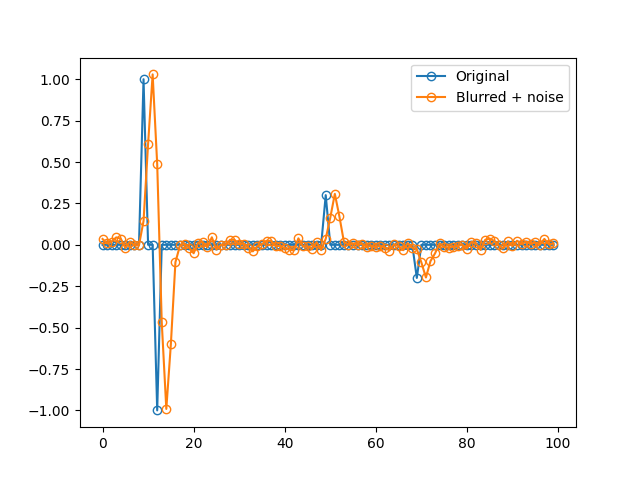
\includegraphics[width=0.6\linewidth]{Images/verify.png}
    \captionof{figure}{Plot of original and blurred+noisy signals}
    \label{figure:blur-works}
\end{center}

\section{Problem 2}

Figure \ref{fig:opt1} shows code which formulates and solves the given optimization
problem. Figure \ref{figure:plot-opt-solution} shows a plot of the deblurred solution.

\begin{center}
\begin{python}
import cvxpy as cp

B_explicit = implicit2explicit(blur, N)
eps = sigma * np.sqrt(N)

x = cp.Variable(N)
objective = cp.Minimize(cp.norm(x, p=1))
constraints = [cp.norm(B_explicit @ x - y, p=2)**2 <= eps**2]
problem = cp.Problem(objective, constraints)
result = problem.solve()

\end{python}
\captionof{figure}{Optimization Solution}
\label{fig:opt1}
\end{center}

\begin{center}
    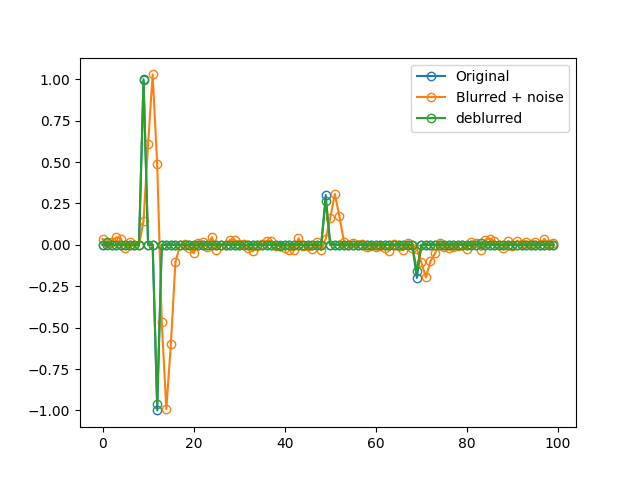
\includegraphics[width=0.6\linewidth]{Images/deblurred.png}
    \captionof{figure}{Plot of original, blurred+noisy signals, and the deblurred signal (optimization solution)}
    \label{figure:plot-opt-solution}
\end{center}

\section{Problem 3}
Figure \ref{fig:opt2} solves the equivalent unconstrained problem using the 
dual value associated with the constraints of Problem 2. We verify the
solutions are the same by taking the 2-norm of their difference. As seen by the
output, they agree within 5 decimal places.

\begin{center}
    \begin{python}
# Problem reformulation using dual variable.
x1 = cp.Variable(N)
lambda_ = constraints[0].dual_value
objective_unconstrained = cp.Minimize(
    cp.norm(x1, p=1) + lambda_ * cp.norm(B_explicit @ x1 - y)**2
)
problem1 = cp.Problem(objective_unconstrained)
problem1.solve()
print(np.linalg.norm(x1.value - x.value))

>>> 1.2942472780651364e-06
    \end{python}

\captionof{figure}{Equivalent Unconstrained Optimization Solution}
\label{fig:opt2}
\end{center}


\section{Problem 4}


The adjoint operator is implemented in the code contained
in figure \ref{fig:adjoint}. We utilize the fact that
the adjoint of the FFT operator is the iFFT (times a scaling factor
which cancels). The adjoint of the operator $\mathcal{H}$ simply applies
element-wise multiplication of the conjugate of $\mathcal{F}(h)$.

\begin{center}
    \begin{python}
def H_adjoint(x):
    h_hat = fft(pad(h, len(x)))
    return x * np.conj(h_hat)


def B_adjoint(x):
    return np.real(ifft(H_adjoint(fft(x))))


    \end{python}
\captionof{figure}{Adjoint Implementation}
\label{fig:adjoint}
\end{center}

Figure \ref{fig:adjoint-test} shows test code which verifies
the inner products $<Ax, y>$ and $<x, A^* y>$ are the same across
range of random vectors. The test passes when taking our implemented blur and blur-adjoint operators
as input.
    
\begin{center}
    \begin{python}

def test_adjoint(A, B, N, M, n_tests=1000):
    # Verify that B is the adjoint of A.
    A_mat = implicit2explicit(A, N)
    B_mat = implicit2explicit(B, M)
    assert A_mat.shape == (M, N), "Matrix representation of  B does not have correct dimensions."
    assert B_mat.shape == (N, M), "Matrix representation of  B does not have correct dimensions."
    for _ in range(n_tests):
        x = np.random.normal(0, 1, N)
        y = np.random.normal(0, 1, M)
        assert np.allclose(
            np.vdot(A_mat @ x, y),
            np.vdot(x, B_mat @ y)
        )

test_adjoint(blur, B_adjoint, N, N)
    \end{python}
\captionof{figure}{Adjoint Test Code}
\label{fig:adjoint-test}
\end{center}

\section{Problem 5}

We use the Lasso Solver that was included with the course materials on GitHub.
To import in the notebook, we downloaded the firstOrderMethods.py file and saved it
in a package titled cvx\_opt, which is accessible from the author's jupyter notebook environment.

Figure \ref{fig:lasso-solver} shows the code which calls the lassoSolver function and compares
the solution to the one computed in Problem 3. The solutions agree within 3 decimal places.


\begin{center}
    \begin{python}
from cvx_opt.first_order_methods import lassoSolver

tau = 1 / (2 * lambda_)
x_direct, solver_info = lassoSolver(blur, y, tau, B_adjoint)

print("Error between solutions: ", np.linalg.norm(x_direct - x1.value))


>>> Iter.  Objective Stepsize
>>> -----  --------- --------
>>>     0  2.06e+00  1.42e-01
>>>   162  1.35e-01  1.42e-01
>>> ==  Quitting due to stagnating objective value  ==
>>> Error between solutions: 0.00040458279990506337
    \end{python}
\captionof{figure}{Optimization using lassoSolver}
\label{fig:lasso-solver}
\end{center}



\end{document}
